\documentclass[11pt,a4paper]{article}

\usepackage[margin=22mm]{geometry}
\usepackage{amsmath,amssymb,booktabs,array,tabularx,longtable}
\usepackage{tikz,pgfplots,xcolor,enumitem,fancyhdr,hyperref}
\pgfplotsset{compat=1.18}
\definecolor{deepblue}{HTML}{267E9A}
\definecolor{warmred}{HTML}{CD715C}
\definecolor{slate}{HTML}{6A7B8C}
\definecolor{lavender}{HTML}{A494B8}
\hypersetup{colorlinks=true,linkcolor=deepblue,citecolor=deepblue,urlcolor=deepblue}
\setlength{\headheight}{15pt}
\pagestyle{fancy}\fancyhf{}\fancyhead[L]{\small NN-native current design: Stage 0}\fancyhead[R]{\small 3 October 2026}\fancyfoot[C]{\thepage}
\setlength{\parskip}{5pt}
\setlength{\emergencystretch}{2em}
\newcommand{\norm}[1]{\left\lVert #1\right\rVert}
\newcommand{\R}{\mathbb{R}}
\newcommand{\C}{\mathbb{C}}
\newcommand{\Id}{\mathrm{Id}}
\newcommand{\op}[1]{\operatorname{#1}}
\newcommand{\Cov}{\operatorname{Cov}_{12}}
\newcommand{\code}[1]{\texttt{#1}}
\newcommand{\coverageTable}{
\begin{center}\small\begin{tabular}{lrrrrr}\toprule
Method & smooth & near-contact & layered & asymmetric & Mean\\\midrule
B0 & 0.9689 & 0.3528 & 0.9198 & 0.6589 & 0.7251 \\
B1 ($s=02$) & 0.9317 & 0.5809 & 0.9010 & 0.7647 & 0.7946 \\
B1 ($s=03$) & 0.9658 & 0.8326 & 0.3139 & 0.8541 & 0.7416 \\
B1 ($s=04$) & 0.9760 & 0.5426 & 0.9379 & 0.9287 & 0.8463 \\
B2 & 0.9718 & 0.5178 & 0.9852 & 0.6751 & 0.7875 \\
B3 & 0.7283 & 0.4142 & 0.7644 & 0.5969 & 0.6259 \\
B4 & 1.0000 & 1.0000 & 1.0000 & 1.0000 & 1.0000 \\
B5 & 1.0000 & 1.0000 & 1.0000 & 1.0000 & 1.0000 \\
\bottomrule\end{tabular}\end{center}}
\newcommand{\coverageFig}{
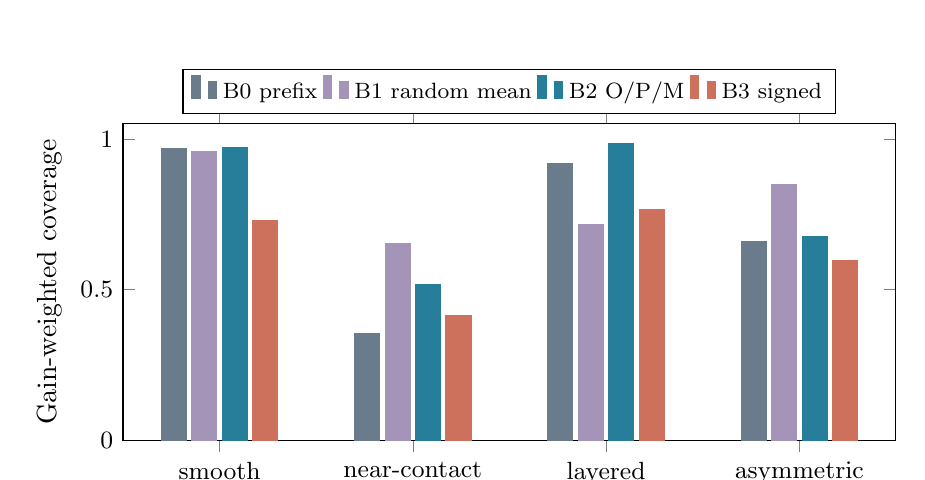
\begin{tikzpicture}\begin{axis}[width=.94\linewidth,height=5.6cm,ybar,bar width=9pt,ymin=0,ymax=1.05,xmin=-.5,xmax=3.5,
xtick={0,1,2,3},xticklabels={smooth,near-contact,layered,asymmetric},ylabel={Gain-weighted coverage},
legend style={at={(.5,1.03)},anchor=south,legend columns=4,font=\footnotesize},tick label style={font=\small}]
\addplot[fill=slate,draw=slate] coordinates {(0,0.96892621) (1,0.35281852) (2,0.91981014) (3,0.65892407)};
\addplot[fill=lavender,draw=lavender] coordinates {(0,0.95783071) (1,0.65206036) (2,0.71758396) (3,0.84914981)};
\addplot[fill=deepblue,draw=deepblue] coordinates {(0,0.97184706) (1,0.51782080) (2,0.98516681) (3,0.67505852)};
\addplot[fill=warmred,draw=warmred] coordinates {(0,0.72834963) (1,0.41419167) (2,0.76436052) (3,0.59686521)};
\legend{B0 prefix,B1 random mean,B2 O/P/M,B3 signed}
\end{axis}\end{tikzpicture}}
\newcommand{\marginFig}{
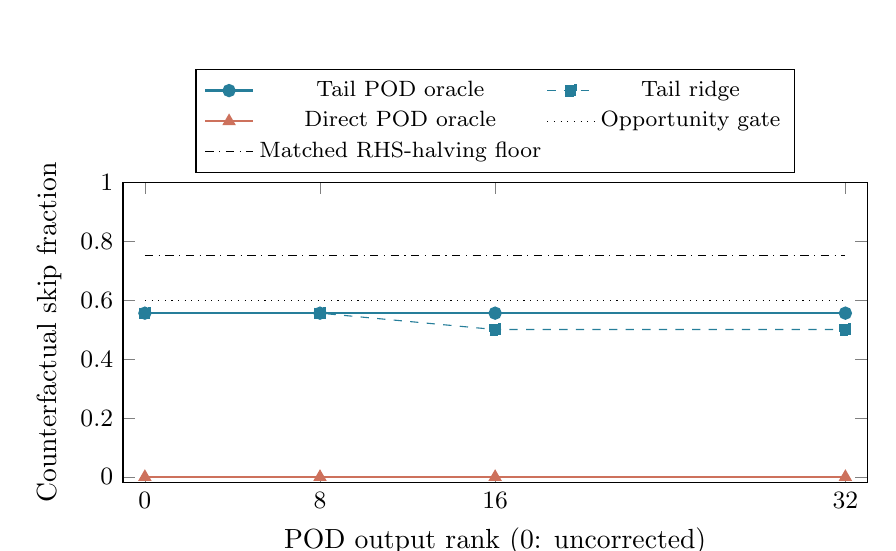
\begin{tikzpicture}\begin{axis}[width=.91\linewidth,height=5.4cm,xmin=-1,xmax=33,ymin=-.02,ymax=1,
xtick={0,8,16,32},xlabel={POD output rank (0: uncorrected)},ylabel={Counterfactual skip fraction},
legend style={at={(.5,1.03)},anchor=south,legend columns=2,font=\footnotesize},tick label style={font=\small}]
\addplot[deepblue,thick,mark=*] coordinates {(0,.55556)(8,.55556)(16,.55556)(32,.55556)};
\addplot[deepblue,dashed,mark=square*] coordinates {(0,.55556)(8,.55556)(16,.5)(32,.5)};
\addplot[warmred,thick,mark=triangle*] coordinates {(0,0)(8,0)(16,0)(32,0)};
\addplot[black,dotted,mark=none] coordinates {(0,.6)(32,.6)};
\addplot[black,dashdotted,mark=none] coordinates {(0,.75)(32,.75)};
\legend{Tail POD oracle,Tail ridge,Direct POD oracle,Opportunity gate,Matched RHS-halving floor}
\end{axis}\end{tikzpicture}}
\setlength{\parindent}{0pt}

\title{Can Neural Current Proposals Outperform Cheap Physics?\\An Offline Feasibility Study for Maxwell Current Design}
\author{Stage 0 research record}
\date{3 October 2026}
\begin{document}\maketitle
\begin{abstract}
We study two decision-oriented uses of learning in reduced Maxwell models: proposing dictionary currents before costly endpoint scoring, and correcting the directional observation defect of a reduced model. The study reuses a pinned numerical archive and runs no neural training, new full-wave right-hand sides (RHS), or nonlinear reconstruction. Across four objects and 36 complete receiver queries, a fixed observation/coupling/injection shortlist improves gain-weighted coverage from 0.7251 to 0.7875 but leaves the difficult near-contact case at 0.5178. A signed-transfer heuristic performs worse, at 0.6259. The remaining coverage gap supports a bounded proposal pilot. Compensation has a different outcome: only two Gaussian objects have complete matched vector labels. With a train-only proper orthogonal decomposition (POD) basis, the primary near-contact test yields 10/18 counterfactual skipped checks for anchor-tail ranks 8, 16 and 32, identical to the uncorrected anchor. The direct-defect oracle yields 0/18. Initialization raises the matched total-RHS-halving requirement to 75\%. We therefore recommend the candidate pilot and withhold a compensation training recommendation. Missing voxel labels and the negative Gaussian representation diagnostic are recorded separately.
\end{abstract}

\section{Research question and decision unit}
A reduced current model replaces a large Maxwell solve by a Galerkin solve in a selected current subspace. Its value for inversion depends on the material step it produces, rather than solely on how much observation energy its currents carry. We ask whether a learned candidate generator has useful opportunity after cheap physical screening, and whether an existing directional-defect representation is accurate enough to preserve actual gain margins.

A \emph{query} is one frozen physical state, receiver current selection, shared material step and anchor. A \emph{move} replaces one original dictionary atom by one incoming atom. The \emph{anchor} is a richer, already constructed reduced current model used to score shortlisted moves. These terms define a local decision problem; the one-swap teacher measures the best feasible move in this dictionary, with no-op available. It does not solve unrestricted current or material optimization.

Learning small current corrections has prior art in induced-current learning~\cite{wei}; SOM-Net combines learned current updates with analytical material updates~\cite{som}. Explicit operator correction~\cite{lunz}, derivative compression~\cite{dino}, and residual correction~\cite{residual} also predate this study. Our contribution here is an evidence-backed feasibility decision with physical input boundaries, complete local teachers and margin-aware costs. A search with three formulations encountered five HTTP 429 operation failures; seven selected bibliographic records resolved. This is a scoped prior-art audit, without a global novelty claim. The recent PEC surface-current graph paper associated with DOI 10.1109/TAP.2025.3602467 remains a full-text audit gap.

\section{Physical and information contract}
Let $L$ denote the full complex Maxwell current operator, $S$ the observation map, and $B_p$ the material-to-current tangent map for illumination $p$. The identities assume an invertible full operator and admitted nonsingular compressed blocks. All six illuminations share one real material vector. For a current basis $U$,
\begin{align}
 R_U&=U(U^*LU)^{-1}U^*, &J_U&=\op{realify}\{SR_UB_p\}_{p=1}^6,\\
 I_{U,p}&=(I-LR_U)B_p, &O_U&=S(I-R_UL).
\end{align}
The complex $L$ and Schur blocks are not assumed Hermitian or positive definite. The archived stability tolerance is $10^{-10}$; no jitter is used. Atom deletion refers to the original physical dictionary ID, even when SVD or QR changes the coordinates used to represent its span.

The saved public arrays are $\widetilde L=Q^*LQ$, $\widetilde S=SQ$, and $PB_p=Q^*B_p$, with a 128-dimensional current embedding $Q$. Their inverse cannot produce full-physics truth. We use them for reduced endpoint calculations and public features. The saved orthonormal physical material tangent, its fingerprint, $\ell$ and $\Lambda=\lambda_{\rm total}I$ remain coupled. The archived total regularization includes prior precision and Levenberg--Marquardt (LM) damping: for smooth early, $\lambda_{\rm total}=10^{-5}+10^{-2}=0.01001$. It is retained in both the step and frozen gain. Gaussian material dimension is 54 real coordinates, voxel dimension 3456. Complex material coordinates are packed as $[\Re c;\Im c]$; observations are packed illumination-major as $[\Re y_p;\Im y_p]$, giving 1536 real data entries. Illumination stacking does not create six independent material steps.

The shared receiver step $x$ minimizes the frozen reduced quadratic. With material-to-observation Jacobian $J_U$, its Gauss--Newton (GN) equation is
\[
 x=-(J_U^TJ_U+\Lambda)^{-1}(J_U^Tr+\ell).
\]
The proposal interface receives F0 cached public signatures and F1 inexpensive projected physical features. Teacher utility and vector labels are separate interfaces. Actual child steps and complete anchor gains (F2) are used only after a shortlist; full Jacobians, reference steps, truth and full gains (F3) remain on the evaluator side. Object identity, geometry category, path and seed are partition/provenance metadata, not learner features.

\section{Complete archive and frozen comparisons}
We use commit \code{56097653e6a814399581c3759fc3e3e8f0c2284c} of the \href{https://github.com/migodam/a17-maxwell-certified-exchange/tree/56097653e6a814399581c3759fc3e3e8f0c2284c}{pinned archive}. Public output hashes and original source hashes are checked against their respective manifests. The raw teacher files are separately checked against the original dataset manifest. Public metadata rewrites can change JSON bytes, so raw and public hashes are not conflated.

The four objects are smooth, near-contact, layered and asymmetric. Each has early, middle and late frozen states with $k=4,8,16$: 36 queries in total. Query identity contains object/state/pool hashes, original selected IDs, the public step hash, anchor, prior, gauge and receiver/operator layout. It avoids collapsing distinct zero-contrast states with equal contrast hashes. Every query contains its full $k(154-k)$ one-swap dictionary: 47,712 unique moves, 43,108 feasible moves and 5208 incoming utility labels. No duplicate canonical move remains. These are correlated local records from four physical objects, not tens of thousands of independent scenes.

For incoming atom $i$, the teacher is
\begin{equation}
t_i(q)=\max\!\left(0,\max_{a\in U_q,\;\mathrm{feasible}} Q_{q,a,i}\right).
\end{equation}
All feasible maximizing drops within the numerical tolerance are retained, and zero-positive cases retain no-op. All 36 archived queries have a gain above their floor; no-op is available but never optimal in this cohort.

\subsection{The six opponents}
B0 is the original family-prefix round-robin selection of twelve incoming atoms. B1 matches those family counts with random draws, using frozen seeds 20261002/03/04. B2 cyclically takes the next unused candidate from descending observation, coupling and material-injection lists, filling exactly twelve. B3 greedily maximizes query-normalized signed-transfer rank minus a fixed 0.25 observation-overlap penalty. B4 uses the already paid full-dictionary endpoint/anchor scores. B5 is the high-fidelity one-swap teacher with no-op.

To define B2/B3, use the projected public operators and receiver $U$. Set
\begin{align}
 \bar c_i&=c_i-U(U^*LU)^{-1}U^*Lc_i,&Y_i&=S\bar c_i,\\
 \gamma_i&=c_i^*L\bar c_i,&n_{p,i}&=c_i^*(I-LR_U)B_p x.
\end{align}
Here and below this feature computation uses the saved projected maps, while the full-operator equations explain the mechanism. The three nonnegative axes are
\begin{align}
 O_i&=\norm{Y_i}^2/\norm{c_i}^2,\\
 P_i&=(\norm{U^*Lc_i}^2+\norm{c_i^*LU}^2)/\norm{c_i}^2,\\
 M_i&=\sum_p|n_{p,i}|^2/(\norm{x}^2\norm{c_i}^2).
\end{align}
B3 forms $w_i=\op{realify}\{Y_i\gamma_i^{-1}n_{p,i}\}_p$ and
\begin{equation}
s_i=-(r+J_Ax)^Tw_i-\tfrac12\norm{w_i}^2.
\end{equation}
This is an addition response at the public receiver step, not the finite material gain of a swap. Percentile ranks are computed within each query. The diversity penalty uses squared normalized $Y_i^*Y_j$ overlap. Numerical ties are fixed at relative $10^{-12}$ score resolution and resolved by original atom ID. A scalar $\gamma$ has usual condition number one; normalized $|\gamma|$ and retained-core reciprocal condition are tracked instead.

\section{Proposal results and mechanism}
Gain-weighted coverage is
\begin{equation}
 \Cov=\frac{\sum_q\max(0,\max_{a,i\in P_q}Q_{q,a,i})}
 {\sum_q\max(0,\max_{a,i\in D_q}Q_{q,a,i})}.
\end{equation}
An absent denominator would be NA. Object means give the four objects equal weight. Top-one recall asks whether the pool contains a maximizing incoming atom; top-four recall averages the fraction of tied top-four incoming labels captured. Gain regret is the full-dictionary best positive gain minus the pool's best positive gain, in the saved objective units.

\coverageTable
\noindent B1 seed suffixes 02/03/04 mean 20261002/03/04. B4 and B5 have coverage one because their pools contain the full dictionary; their decision roles and costs differ.
\begin{figure}[htbp]\centering\coverageFig
\caption{Cheap screening leaves opportunity in the difficult objects. Random bars show the three fixed-seed mean; all individual seeds appear in the table. These are descriptive values, not confidence intervals.}\end{figure}

B0 reproduces the reported 0.969/0.353/0.920/0.659 bottleneck. The full-dictionary anchor top-one capture is 0.9960/0.9810/0.9937/0.9883, confirming that accurate ranking is available after a useful atom reaches the scored pool. B2 increases near-contact coverage by 0.1650 and layered coverage by 0.0654, but near-contact 0.5178 and asymmetric 0.6751 remain below 0.70 and 0.85. Its equal-object mean 0.7875 also misses 0.85.

B3's mean 0.6259 is a substantive negative result. The public receiver-direction addition response does not capture the changed material GN step or the deletion-dependent retained core. Observation diversity cannot repair that mismatch by itself. This supports targeting incoming utility directly rather than assuming a signed addition surrogate ranks material swaps.

The strongest single frozen cheap comparison has mean 0.8463 (B1, seed04), leaving 0.1537 to the one-swap teacher. That seed still fails the near-contact gate. Another seed improves near-contact but collapses layered coverage. Choosing a different seed after observing each object or query would create an unearned oracle. None of the fixed cheap opponents meets all three elimination gates. The remaining gap justifies a bounded candidate pilot; it does not show a neural model can learn the gap.

\begin{table}[htbp]\centering\small
\caption{Recall and summed gain regret. All objects have nine queries and zero no-positive queries. Complete B1 rows and every query are in the delivered CSVs.}
\begin{tabular}{llrrr}\toprule Object & Method & Top1 & Top4 & Regret sum\\\midrule
smooth & B0 & 0.222 & 0.111 & 4.79e-05 \\
smooth & B2 & 0.222 & 0.167 & 4.34e-05 \\
smooth & B3 & 0.000 & 0.000 & 4.18e-04 \\
smooth & B4 & 1.000 & 1.000 & 0.00e+00 \\
near-contact & B0 & 0.000 & 0.000 & 1.94e-04 \\
near-contact & B2 & 0.111 & 0.083 & 1.45e-04 \\
near-contact & B3 & 0.000 & 0.028 & 1.76e-04 \\
near-contact & B4 & 1.000 & 1.000 & 0.00e+00 \\
layered & B0 & 0.222 & 0.250 & 2.08e-04 \\
layered & B2 & 0.444 & 0.278 & 3.85e-05 \\
layered & B3 & 0.000 & 0.028 & 6.11e-04 \\
layered & B4 & 1.000 & 1.000 & 0.00e+00 \\
asymmetric & B0 & 0.000 & 0.056 & 1.77e-04 \\
asymmetric & B2 & 0.000 & 0.111 & 1.69e-04 \\
asymmetric & B3 & 0.000 & 0.000 & 2.09e-04 \\
asymmetric & B4 & 1.000 & 1.000 & 0.00e+00 \\
\bottomrule\end{tabular}\end{table}

F1 components are measured separately. Their joint warm median is 4.60 ms/query, using already cached projected maps. Child endpoint scoring remains a post-shortlist cost. These timings do not include acquiring a physical workspace or establishing a full-wave reference, and are not an end-to-end acceleration result.

\section{Compensation: lawful labels before architecture}
For the same legal material difference $d$, we compare
\begin{equation}
 \Delta z_U=(J_F-J_U)d=(J_A-J_U)d+(J_F-J_A)d.
\end{equation}
The known inner correction is not learned. The richer anchor tail is the remaining target. $A$ and $U$ need not be nested; a smaller empirical tail is not a monotonicity theorem.

Gaussian $\code{fullJ}$ gives legal measurement labels for 101 smooth and 103 near-contact matched directions. Voxel $V/\code{fullJV}$ contains only sixteen material directions. The tested voxel differences have relative projection residual 0.9948--0.9992, far above $10^{-9}$. We also inspect every stored endpoint step and full $Js$. Only the asymmetric late $k=8$ receiver can be recovered in the lawful saved snapshot span, giving one matched difference vector. The other 194 voxel matched vectors remain missing. A scalar gain does not determine $J_Fd$.

There are zero full-current or unresolved-current labels. Measurement outputs cannot identify current components in the observation nullspace; a full solve in public $Q$ coordinates would still be a reduced model. The one voxel vector is an inventory finding, excluded from object-level B fitting and claims.

Median anchor-tail/direct-defect norm ratios are 0.3729 (smooth) and 0.4356 (near-contact). Removing the inner correction substantially reduces target magnitude. Accuracy for a decision, however, depends on residual orientation and margin, not merely target size.

\subsection{Train-only POD, fixed ridge and source oracle}
POD (proper orthogonal decomposition) is the left singular basis of uncentered training defect snapshots. We freeze output ranks 8/16/32, preserving a zero-input linear correction. Ridge uses a fixed training-RMS scaler, no intercept and $\alpha=10^{-6}\sigma_{\max}(H)^2$. It is a shared state-blind linear baseline, not an implemented state-conditioned Maxwell-native network.

The prescribed object cycle has 18 train, nine validation and nine test queries per fold. In Fold1, smooth provides 101 training directions and near-contact 103 test directions; layered validation lacks complete vectors. Fold0 has no complete Gaussian training object. In Fold3, near-contact trains and smooth is validation, not a second test. We do not move validation into training to manufacture a two-way test. Thus B is a two-object diagnostic with one available prescribed primary test fold, not a four-object result.

The source encoder uses a fixed random physical-row sketch of the \emph{projected} anchor injection, shared across the verified common Gaussian physical grid. At 8/16/32 complex rows per illumination it has 96/192/384 real features. For the saved 54-dimensional Gaussian gauge, its numerical rank is 54 in all cases. Using the evaluation-side full Jacobian, the state-specific unobservable-tail residual is at most $4.47\times10^{-15}$ relative. This tests $\ker H\subseteq\ker(J_F-J_A)$ on that gauge. It does not furnish a public correction operator or resolve off-$Q$ current labels. Voxel source sufficiency cannot be inferred from this Gaussian result.

\section{Gain margins and initialized verification cost}
For a fixed material difference $d$ and exact archived evaluator output $u=r+J_Fx$,
\begin{equation}
 Q=-u^Tz-(\ell+\Lambda x)^Td-\tfrac12(\norm{z}^2+d^T\Lambda d),\qquad z=J_Fd.
\end{equation}
If $e=z-\hat z$, the difference is $-(u+\hat z)^Te-\norm{e}^2/2$. Hence $|Q-\hat Q|\leq v\epsilon+\epsilon^2/2$ for $v=\norm{u+\hat z}$ and $\norm{e}\leq\epsilon$. For positive predicted margin $m=\hat Q-\tau$,
\begin{equation}
\epsilon_{\rm crit}=\frac{2m}{\sqrt{v^2+2m}+v}.
\end{equation}
Here $\hat Q$ substitutes $\hat z$ in the displayed gain while retaining exact evaluator $u$. It differs from the anchor score used for A, whose residual is $r+J_Ax$. The stable expression avoids subtracting two nearly equal terms. We label a check counterfactually skippable only when the actual saved response error is below this threshold. All 18 primary B4 finalists have true gain above their floor.

\begin{figure}[htbp]\centering\marginFig
\caption{Primary near-contact test, B4's 18 matched finalists. Tail POD projection improves residuals but adds no skipped checks over the uncorrected anchor. Direct-defect POD yields zero. The 60\% opportunity gate and 75\% initialized RHS-halving floor are different requirements.}\end{figure}

Direct-defect POD gives 0/18 at every rank. Anchor-tail POD gives 10/18 at every rank, as does the uncorrected anchor. Tail ridge gives 10/18 at rank8 and 9/18 at ranks16/32. For B2's matched finalists, rank32 tail POD gives 7/18. The rank32 B4 median tail-relative error is 0.8868; its median error-to-critical-radius ratio is 0.5413. A median below one does not imply that enough finalists cross the gate. The reversed Gaussian cohort is Fold3 validation; its tail POD skip fraction is 8/18 at all ranks.

This projection oracle uses optimal coefficients for Euclidean response approximation in the fixed training basis. It is not a universal maximizer of the number of margin-certified decisions. The negative result applies to the tested POD/ridge pipeline and does not exclude every possible state-conditioned representation.

Let initialization cost be $I$ full RHS and matched finalist checks cost $R$ RHS, with skip fraction $\rho$. Before model overhead,
\begin{equation}
 C_{\rm new}=I+(1-\rho)R+C_{\rm refresh}+C_{\rm audit}+C_{\rm failed}.
\end{equation}
If the additional terms vanish, total RHS halving needs $\rho\geq(1+I/R)/2$. Historical 1164 finalist RHS and 216 initialization RHS give 59.28\%. Our single-decision test has $I=54$, $R=108$, requiring 75\%. The observed 55.6\% oracle opportunity gives an ideal initialized RHS ratio 0.6296. Cold setup, model/source computation, refresh and audits increase costs. These fullJ/table reuses create no actual skipped physical solve or measured speedup. Archived high-fidelity labels and this exact-error diagnostic are not deterministic physical error certificates; certified ROM methods require their own error controls~\cite{cert}.

\section{Verification, reproducibility and retained failures}
We wrote 128 fresh non-Hermitian complex algebra cases for the two-sided defect, Schur tail, non-nested anchor decomposition, phase covariance, original-ID permutation and gain-error bound. The largest identity residual is $9.69\times10^{-16}$; no tested gain bound is violated. On one early $k=8$ query per object, phase/permutation actions, public forbidden-field canaries and real linearity checks pass. Ridge zero/scaling/additivity and prediction canaries are separate checks. No neural architecture has been implemented or tested.

The supplied folder lacks the original validation script, original configuration/results and separate reference file. References were restored from the merged reading version. The new checks are equivalent audits, not reproduction of the original reported 128 PASS result. Parser, SVD-gauge tester, adapter and serialization failures are retained with their costs. Sixteen upstream Woodbury units crossed the unchanged $10^{-10}$ normal-residual gate; one fixed residual correction of the same normal equation validates them below the gate. Vendor code, physical operators and $\lambda$ are unchanged. This is a numerical validation repair, not a proposed solver or speed experiment.

The reproduction package contains source hashes, frozen configuration, query/move identities, all seed comparisons, matched vector provenance, fitted bases, source oracles, failure/claim/reference ledgers and replot scripts. All new artifacts reside under \code{A18\_NN\_NATIVE}. Single-process resource receipts include failed attempts; peak memory remains below 4 GiB and numerical CPU below one hour.

\section{Independent decisions and stopping point}
\textbf{A: GO to a bounded tiny pilot, as a recommendation only.} No fixed cheap opponent closes the difficult-object gap. A future student must attain near-contact coverage 0.70, asymmetric 0.85 and mean 0.85, then exceed the strongest cheap mean by 0.05 or halve cost at quality within 0.01. Shared MLP, Set Transformer, ordinary GAT and phase-consistent physics-edge GNN configurations share inputs, twelve candidates, at most 200k parameters, 60 epochs, four object folds and two seeds. They remain disabled.

\textbf{B: globally data-incomplete; no training recommendation from the tested Gaussian oracle.} Complete Gaussian labels support the smaller-tail mechanism and source-rank diagnostic, but the tested output bases do not add margin/cost opportunity. Four-object B assessment first needs legal matched voxel vectors and receiver outputs. A new representation would need train-only evidence that it changes this margin ceiling, with a fixed-state map linear in $d$ and an explicit cache refresh budget.

Candidate Generator first remains the useful next-stage ordering. A and B have independent gates; A's opportunity does not authorize B training. This study ends after the feasibility artifacts and manuscripts. Training epochs, new full-wave RHS, new nonlinear trajectories, statistical safety calibration, remote execution and publication all remain unperformed.
\appendix\section{Audit entry points}
The nine mandatory files are the inventory, query manifest, object splits, feature costs, analytic baselines, defect-label availability, defect oracle, cost ledger and Stage0 decision. \code{CLAIM\_LEDGER.csv} is the shared evidence index. \code{FUTURE\_TRAINING\_CONFIG.json} is disabled. \code{START\_HERE.md} gives commands and rendering provenance.

\begin{thebibliography}{9}
\bibitem{wei} Z. Wei and X. Chen, ``Physics-Inspired Convolutional Neural Network for Solving Full-Wave Inverse Scattering Problems,'' IEEE TAP, 2019. \href{https://doi.org/10.1109/TAP.2019.2922779}{doi:10.1109/TAP.2019.2922779}. Abstract-level evidence in this study.
\bibitem{som} Y. Liu et al., ``SOM-Net: Unrolling the Subspace-based Optimization for Solving Full-wave Inverse Scattering Problems,'' 2022. \href{https://arxiv.org/abs/2209.03567}{arXiv:2209.03567}. Method and Algorithm 1 inspected.
\bibitem{lunz} S. Lunz et al., ``On Learned Operator Correction in Inverse Problems,'' 2020 preprint. \href{https://arxiv.org/abs/2005.07069}{arXiv:2005.07069}; journal DOI \href{https://doi.org/10.1137/20M1338460}{10.1137/20M1338460}. Sections 3--4 inspected.
\bibitem{dino} T. O'Leary-Roseberry et al., ``Derivative-Informed Neural Operator: An Efficient Framework for High-Dimensional Parametric Derivative Learning,'' 2022 preprint, revised 2023. \href{https://arxiv.org/abs/2206.10745}{arXiv:2206.10745}. Abstract-level evidence.
\bibitem{residual} L. Cao et al., ``Residual-based error correction for neural operator accelerated infinite-dimensional Bayesian inverse problems,'' 2022 preprint. \href{https://arxiv.org/abs/2210.03008}{arXiv:2210.03008}. Abstract-level evidence.
\bibitem{cert} B. Haasdonk et al., ``A new certified hierarchical and adaptive RB-ML-ROM surrogate model for parametrized PDEs,'' 2022. \href{https://arxiv.org/abs/2204.13454}{arXiv:2204.13454}. Abstract-level evidence.
\end{thebibliography}

\end{document}
